\section{Ανάλυση Μεθόδου}
Το πρόγραμμα λειτουργεί με 3 βασικές οντώτητες:
\begin{itemize}
    \item Τον \textbf{Socket Client}. Χρήσιμοποιήται από τον τελικό
        χρήστη. Εδώ ο χρήστης εισάγει τα δεδομένα που είναι απαραίτητα, δηλαδή
        της πληροφορίες διανύσματος (μέγεθος και στοιχεία) και ένα αριθμό
        επιλογών για την επεξεργασία του διανύσματος (οι συγκεκριμένοι αριθμοί
        εισάγονται επαναληπτικά).
    \item Τον \textbf{Socket Server/ RPC Client ή Middleware}. Ουσιαστικά\
        μεσολαβεί στην επικοινωνία των Socket Client και RPC Server, κάνοντας:
\begin{itemize}
        \item Τις απαραίτητες δευσμεύσεις μνήμης.
        \item Τις επεξεργασίες μετάφρασης των δεδομένων του χρήστη προς τον
            RPC Server.
        \item Την μεταβίβαση των πληροφοριών/αποτελεσμάτων από τον Socket
            Server προς τον Socket Client και το αντίθετο.
\end{itemize}
    \item Τον \textbf{RPC Server}. Εκτελεί τις μαθηματικές πράξεις πάνω στο
        διάνυσμα με χρήση των Remote Procedure Calls σε συνεργασία με τον
        RPC Client και στέλνει τα αποτελέσματα στον προαναφερόμενο.
\end{itemize}
\begin{figure}[ht]
    \centering
    \begin{tikzpicture}
        \node (left) at (0,1)   {Socket Client};
        \node (middle) at (6,1) {Socket Server/};
        \node (middledown) at (6,0.5) {RPC Client};
        \node (middledowndown) at (6,0) {(Middleware)};
        \node (right) at (12,1) {RPC Server};
        \draw[->,orange] (left.north)       .. controls +(up:2cm)   and +(left:1cm)    .. node[above,sloped] {\small Διάνυσμα, Επιλογές} (middle.west);
        \draw[->,blue] (middle.north)       .. controls +(up:2cm)   and +(left:1cm)    .. node[above,sloped] {\small Επεξεργασμένες Πληροφορίες} (right.west);
        \draw[->,blue] (middledowndown.south)   .. controls +(down:2cm) and +(right:1.2cm) .. node[below,sloped] {\small Φιλτραρισμένα Αποτελέσματα} (left.east);
        \draw[->,red] (right.south) .. controls +(down:4cm) and +(right:1cm)   .. node[below,sloped] {\small Αποτελέσματα} (middle.east);
    \end{tikzpicture}
    \caption{\footnotesize{Η αρχιτεκτονική του προγράμματος}}
    \label{fig:searx-oper}
\end{figure}
Παραπάνω αρχεία που βρίσκονται στους φακέλους με τον πηγαίο κώδικα είναι
είτε βοηθητικές συναρτήσεις είτε μέρος αυτών των 3 οντωτήτων αλλά χωρισμένες
σε διαφορετικά αρχεία για ευκολία χειρισμού και κατανόησης.
\\
Έχει γίνει προσπάθεια να γίνει πρόληψη για τα σφάλματα του χρήστη, για
παράδειγμα η εσφαλμένη είσοδος δεδομένων με διαφορετικό τύπο από τον ζητούμενο
κ.α.
\section{Ενδεικτικά Τρεξίματα}
Για το compilation του προγράμματος αρκεί η εντολη "make" τον αρχικό κατάλογο του
προγράμματος:
\\
\begin{center}
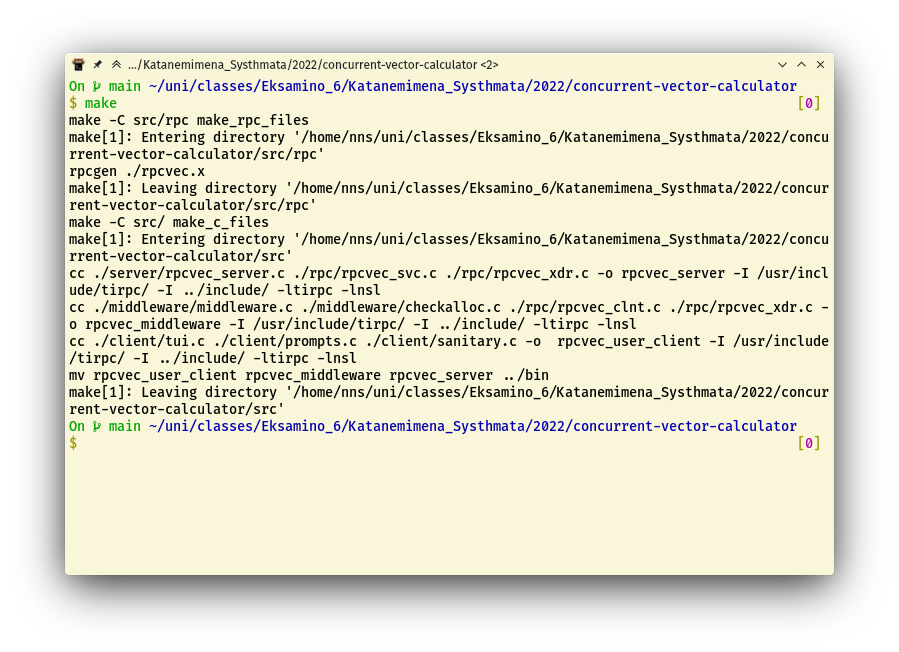
\includegraphics[scale=0.7]{compilation}
\end{center}
Για τνο τρέξιμο εκτελούμε τις εξής εντολές σε σειρά στον αρχικό κατάλογο της
εργασίας (Σε τρία διαφορετικά τερματικά).
\begin{center}
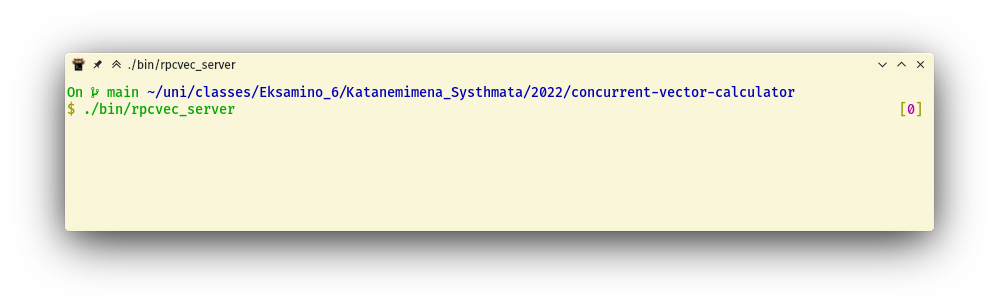
\includegraphics[scale=0.6]{run_step1}
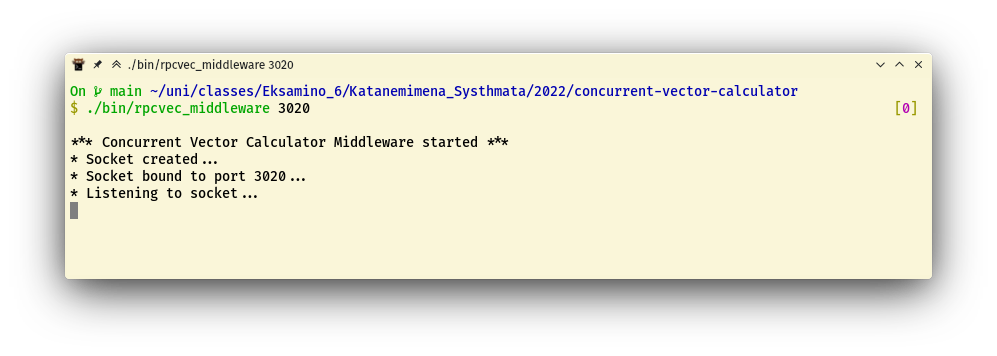
\includegraphics[scale=0.6]{run_step2}
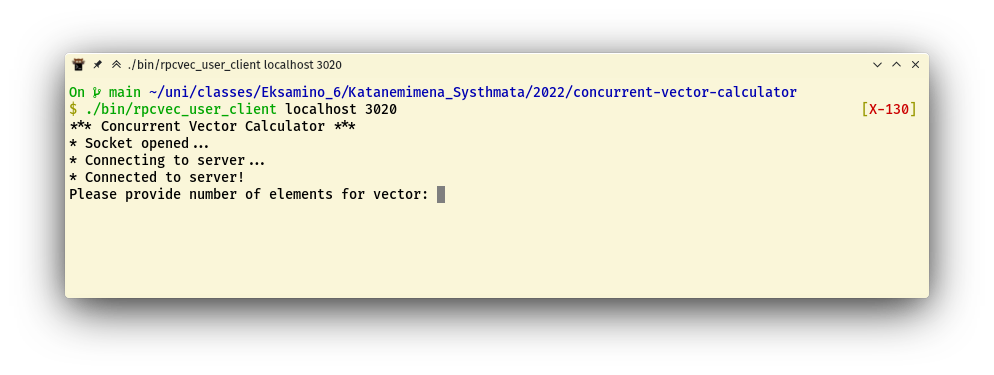
\includegraphics[scale=0.6]{run_step3}
\end{center}
Με την εκτέλεση της τελευταίας εντολής βλέπουμε στο δεύτερο παράθυρό μας ότι
πλέον συνδέθηκε το Middleware με τον Socket Client:
\begin{center}
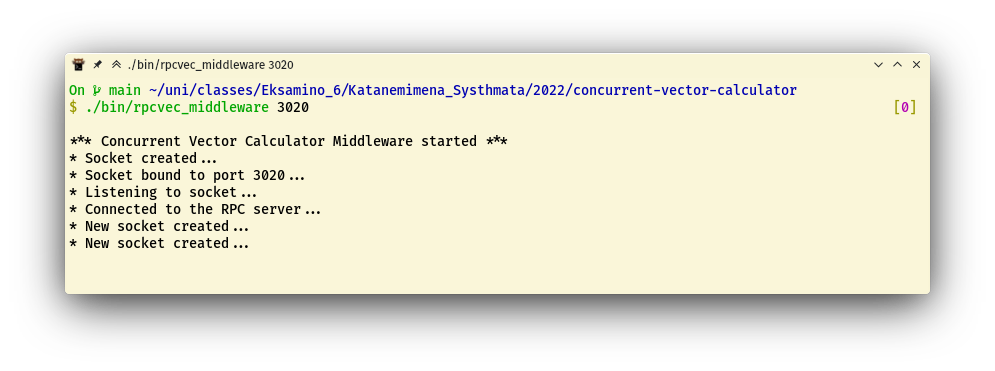
\includegraphics[scale=0.6]{run_step4}
\end{center}
Έπειτα, χρησιμοποιούμε το πρόγραμμα κανονικά με τις ενδείξεις στο τερματικό,
τα τρία παράθυρα κατά την διάρκεια του ενδεικτικού τρεξίματος αυτού είναι σε
κάθε βήμα τις διαδικασίας:
\subsection{Βήμα Πρώτο}
Εισάγουμε τον αριθμό των στοιχείων και τα στοιχεία:
\begin{center}
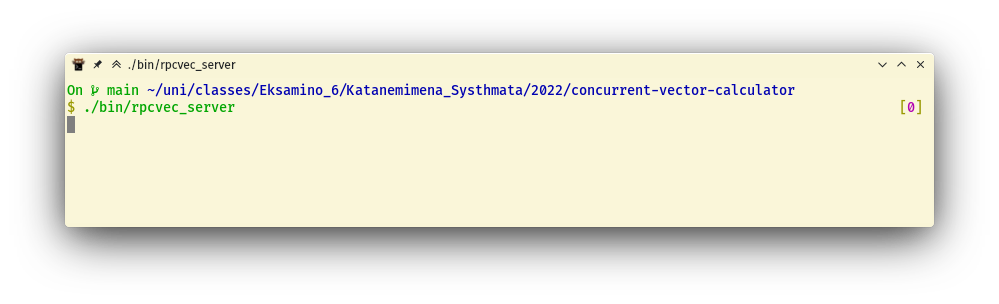
\includegraphics[scale=0.6]{sample_run_step1_1}
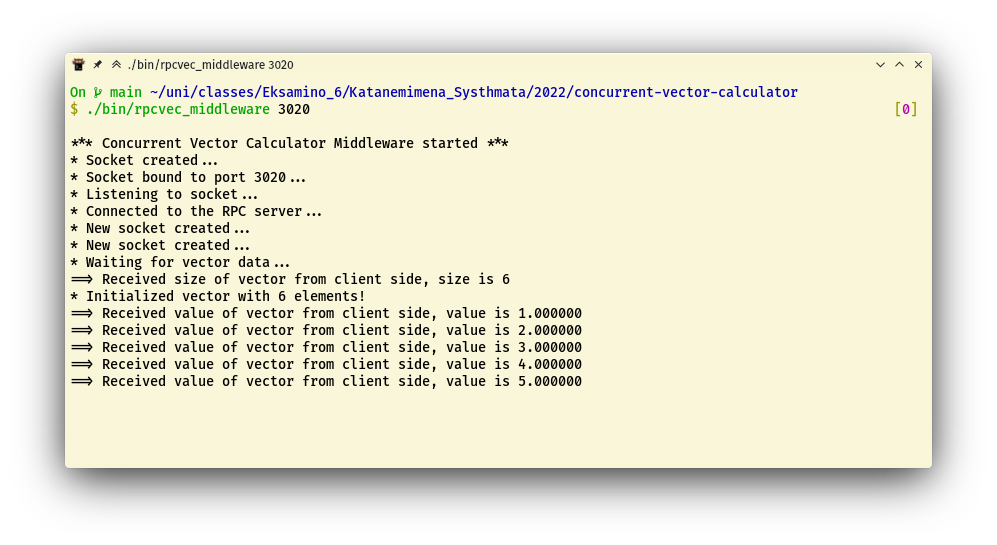
\includegraphics[scale=0.6]{sample_run_step1_2}
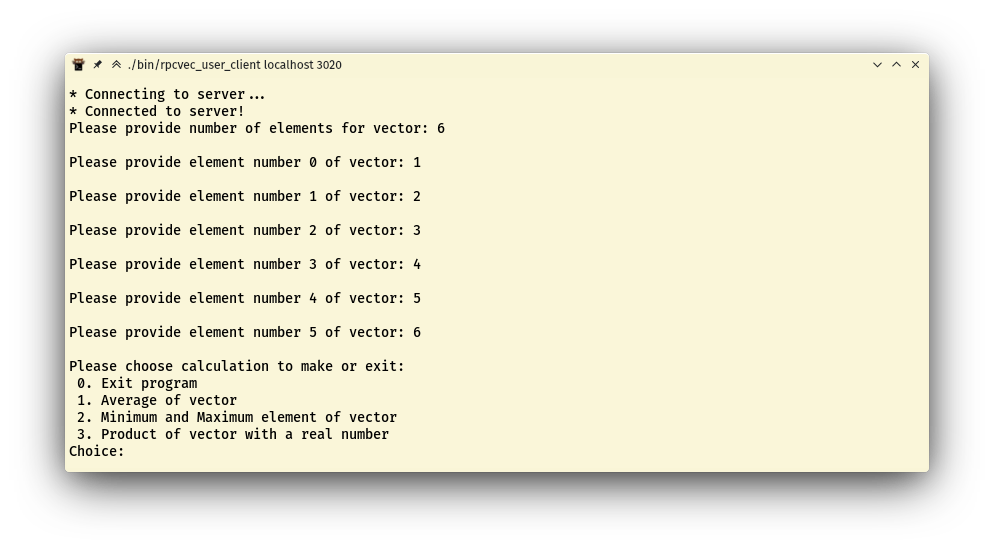
\includegraphics[scale=0.6]{sample_run_step1_3}
\end{center}
\subsection{Βήμα Δεύτερο}
Εισάγουμε 0-3 για να ακολουθήσουμε την αντίστοιχη διαδικασία.
Στο ενδεικτικό τρέξιμο αυτό θα τις επιλέξουμε με σειρά 1,2,3,0.
\\
Επιλέγουμε την 1:
\begin{center}
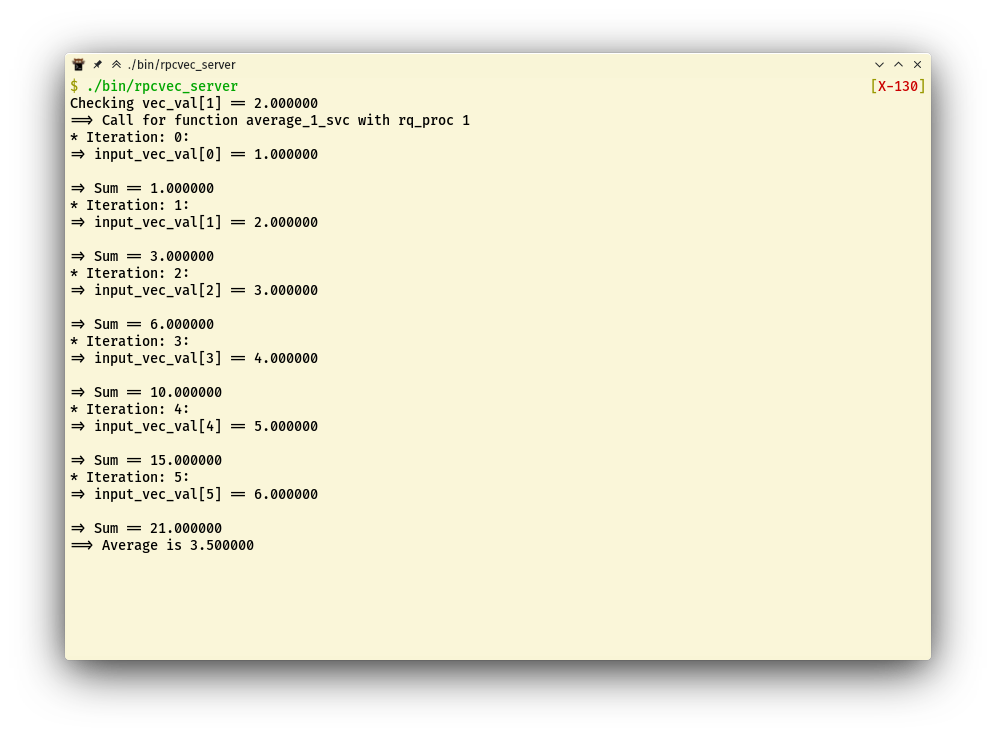
\includegraphics[scale=0.6]{sample_run_step2_3}
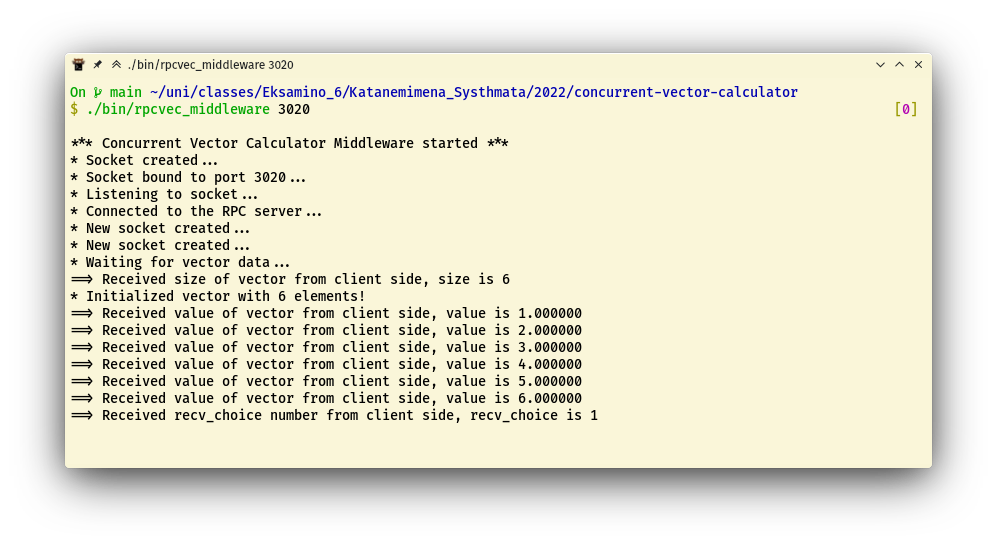
\includegraphics[scale=0.6]{sample_run_step2_1}
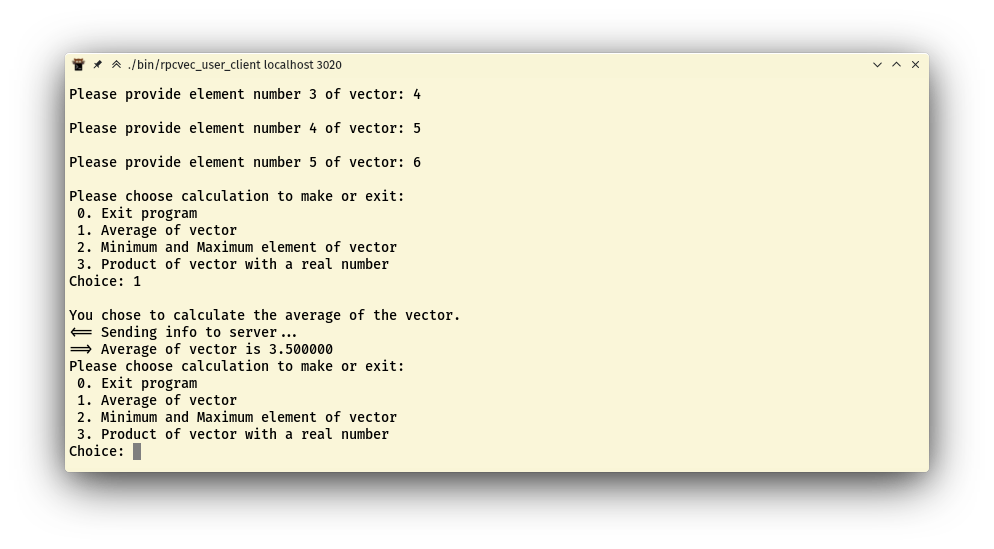
\includegraphics[scale=0.6]{sample_run_step2_2}
\end{center}
Η μέση τιμή του διανύσματος βρέθηκε και εμφανίστηκε σωστά!
Στην συνέχεια, επιλέγουμε την 2:
\begin{center}
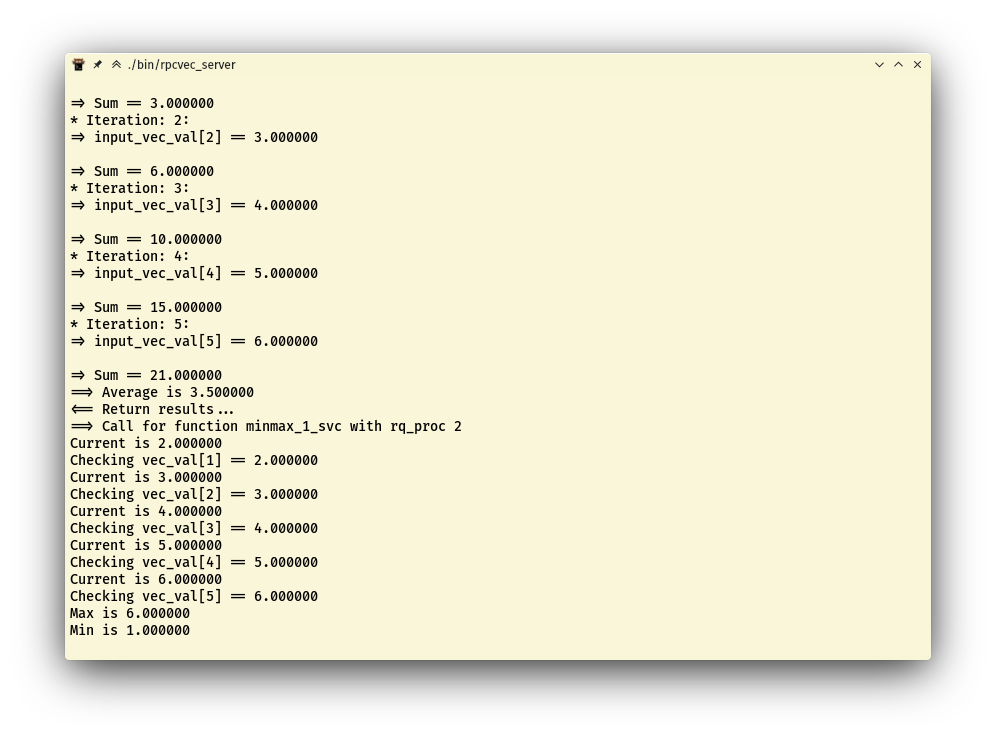
\includegraphics[scale=0.6]{sample_run_step3_3}
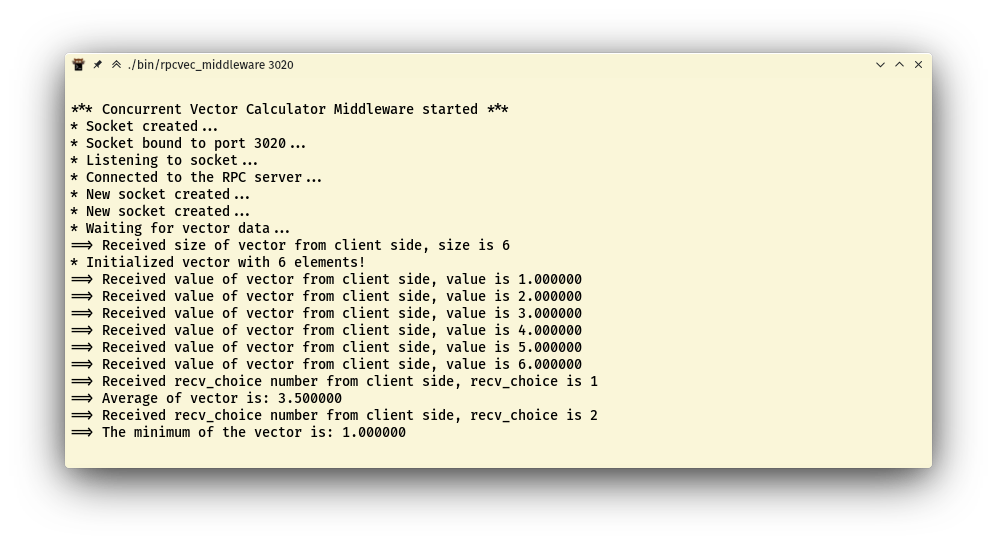
\includegraphics[scale=0.6]{sample_run_step3_1}
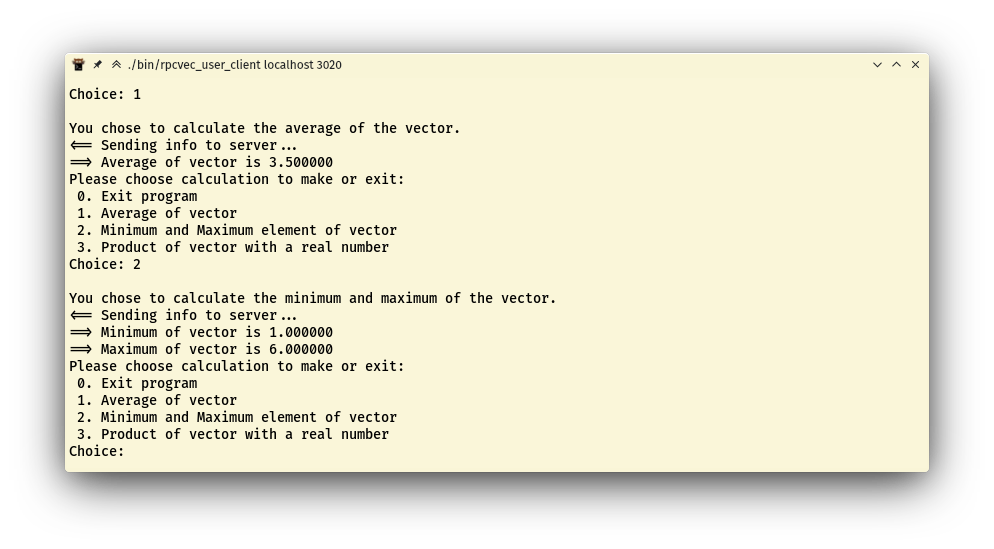
\includegraphics[scale=0.6]{sample_run_step3_2}
\end{center}
Η μέγιστη και ελάχιστη τιμή του διανύσματος βρέθηκε και εμφανίστηκε σωστά!
\\
Στην συνέχεια, επιλέγουμε την 3 και δίνουμε έναν αριθμό:
\begin{center}
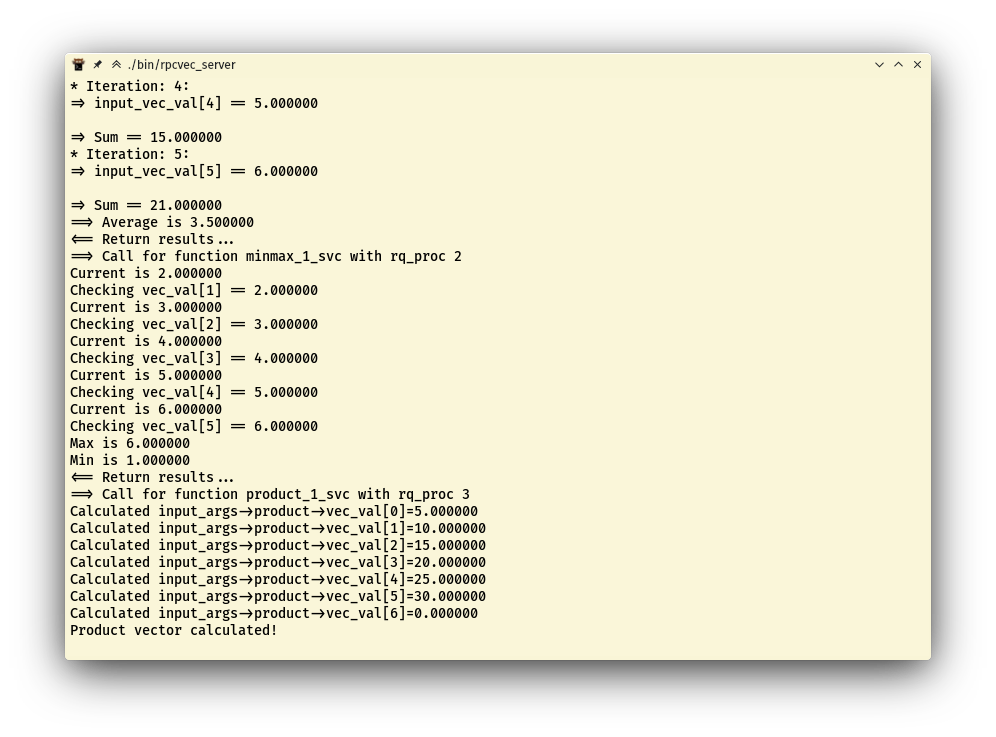
\includegraphics[scale=0.6]{sample_run_step4_3}
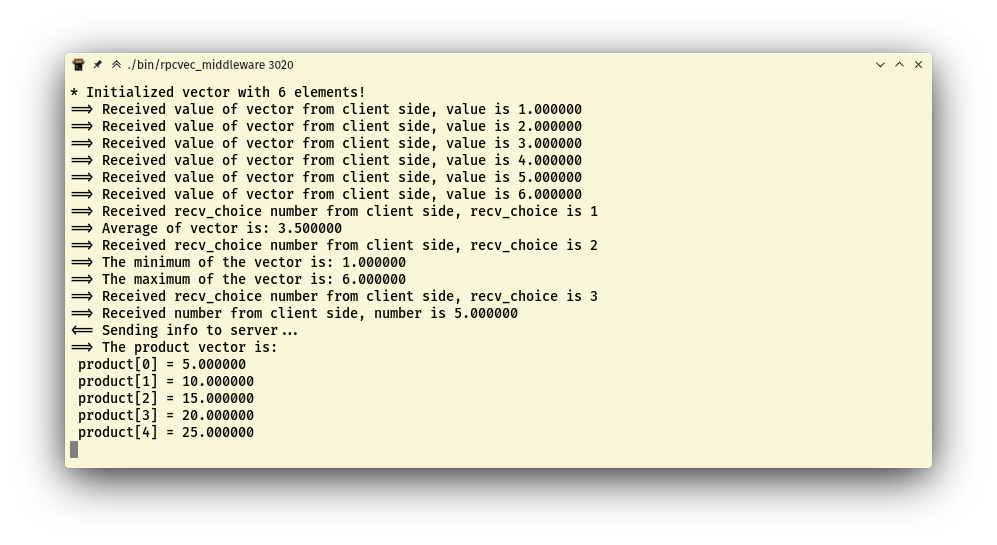
\includegraphics[scale=0.6]{sample_run_step4_2}
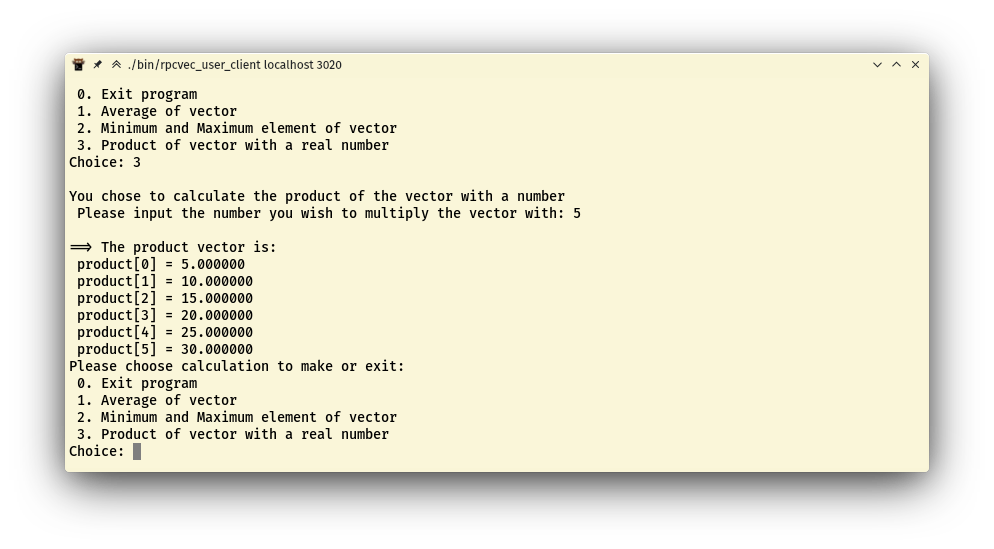
\includegraphics[scale=0.6]{sample_run_step4_1}
\end{center}
Το γινόμενο του διανύσματος με έναν αριθμό βρέθηκε και εμφανίστηκε σωστά!
\\
Στην συνέχεια, επιλέγουμε την 0:
\begin{center}
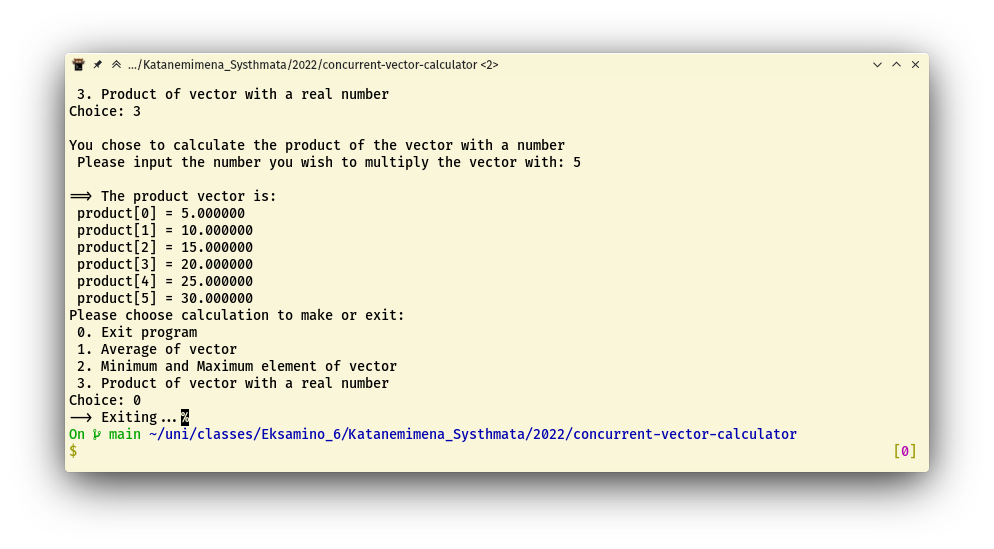
\includegraphics[scale=0.6]{sample_run_step5_1}
\end{center}
Το πρόγραμμά μας τερμάτισε.
